\documentclass[11pt]{article}

\usepackage{amsmath,mathtools,siunitx,amssymb}
\usepackage[a4paper,left=1.5cm,right=1.5cm,top=2cm,bottom=2cm]{geometry}
\usepackage{float,subcaption,graphicx}
\usepackage{enumitem,pifont}
\usepackage{fancyhdr}
\renewcommand{\labelitemi}{\ding{228}}
\renewcommand{\labelitemii}{\ding{229}}
\renewcommand{\labelitemiii}{\ding{225}}
\setlist[itemize]{noitemsep}
\usepackage[dvipsnames]{xcolor}
\usepackage{color,hyperref}
\hypersetup{colorlinks=true}

\graphicspath{{images/}}

\rhead{Last Updated: 15-08-20}

\begin{document}
\thispagestyle{fancy}
{\Large\bfseries Replicating the Oblique Constraints}

\begin{itemize}
    \item Replicating James' work on the obliques has yielded very similar results to his
    \item Figures 1 and 2 compare to his work on Overleaf, and Figure 3 compares to Figure 3 in \href{https://arxiv.org/pdf/2003.03386.pdf}{2003.03386} 
\end{itemize}
\begin{figure}[h]
    \centering
    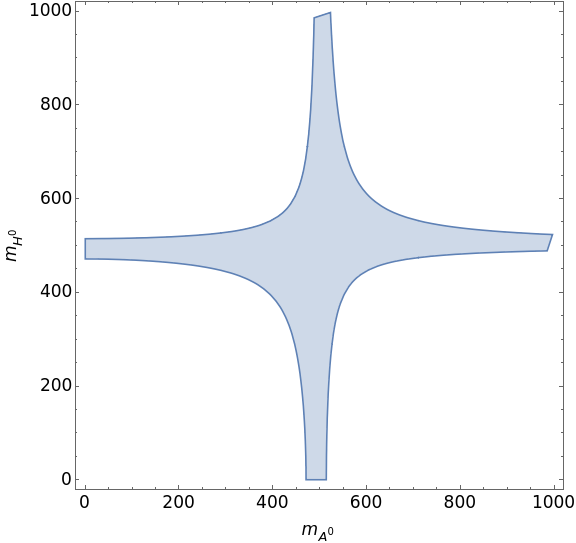
\includegraphics[width=0.4\textwidth]{oblique2D.png}
    \caption{Cross-section in $m_{H^0}-m_{A^0}$ space for $m_{H^+}=500\,$GeV,$\theta=\frac{\pi}{2}$, and assuming $U=0$ at $95\%\,$CL}
\end{figure}
\begin{itemize}
    \item Overall, we see the same results as James has discussed: that it is very closely set that at least one of the new scalar masses must be approximately equal to $m_{H^+}$
    \item There appears to very little difference now between our results and I'm quite happy with my calculations so I'd say we're quite happy to see we're in agreement on these results
\end{itemize}
\begin{figure}[h]
    \centering
    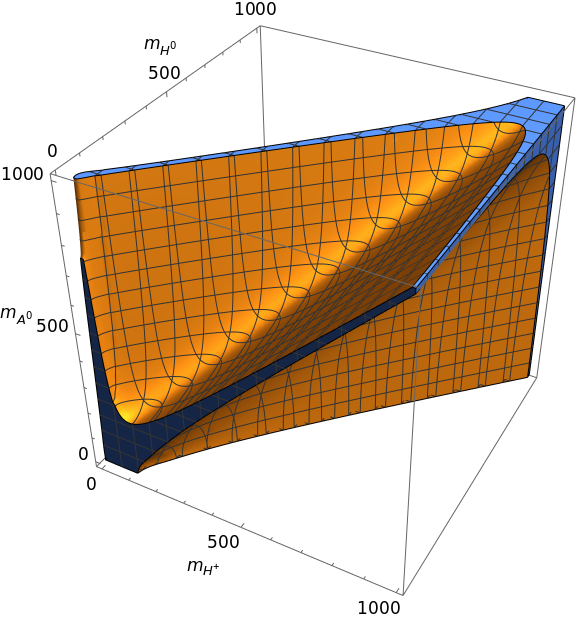
\includegraphics[width=0.4\textwidth]{oblique3D.png}
    \caption{Full scan for $\theta=\frac{\pi}{2}$ and $U=0$ at $95\%\,$CL}
\end{figure}
\newpage
\begin{itemize}
    \item I've managed to quite closely replicate the work of Figure 3 in \href{https://arxiv.org/pdf/2003.03386.pdf}{2003.03386} considering just T, seen in Figure 3 here
    \item We can see that again this favours the scalar masses lying fairly close to $m_{H^+}$, although there is more room for variation than above
\end{itemize}
\begin{figure}[ht]
    \centering
    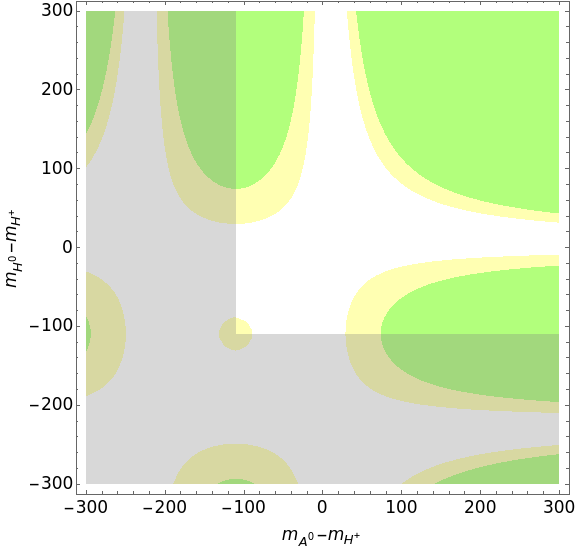
\includegraphics[width=0.4\textwidth]{obliqueT.png}
    \caption{Scalar mass splittings excluded by $T$ for $\theta=\frac{\pi}{2}$ and $m_{H^+}=110\,$GeV at $1\sigma$ (yellow) and $2\sigma$ (blue). The gray region indicates where is forbidden by requiring that $m_{H^0},m_{A^0}>0$.}
\end{figure}
\begin{itemize}
    \item However, this is for $m_{H^+}=110\,$GeV which is smaller than the limits set by direct searches, so in Figure 4, I have tested this again for $m_{H^+}=500\,$GeV
    \item This essentially replicates Figure 1 without the additional constraints of S
\end{itemize}
\begin{figure}[ht]
    \centering
    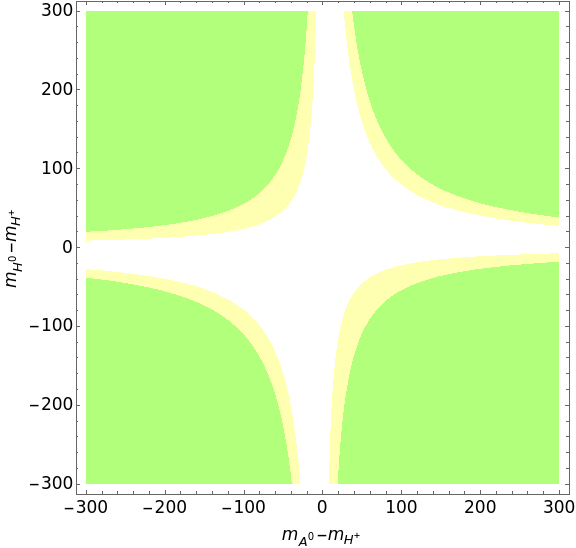
\includegraphics[width=0.4\textwidth]{obliqueT2.png}
    \caption{Scalar mass splittings excluded by $T$ for $\theta=\frac{\pi}{2}$ and $m_{H^+}=500\,$GeV at $1\sigma$ (yellow) and $2\sigma$ (blue).}
\end{figure}

\end{document}

